%!TEX TS-program = xelatex
\documentclass[a4paper,14pt]{article}

% В этом документе преамбула

%%% Работа с русским языком
\usepackage{cmap}					% поиск в PDF
\usepackage{mathtext} 				% русские буквы в формулах
%\usepackage[T2A]{fontenc}			% кодировка
%\usepackage[utf8]{inputenc}			% кодировка исходного текста
\usepackage[english,russian]{babel}	% локализация и переносы
\usepackage{indentfirst}
\frenchspacing

%%%Шрифты
\usepackage{fontspec}      %% подготавливает загрузку шрифтов Open Type, True Type и др.
\defaultfontfeatures{Ligatures={TeX},Renderer=Basic}  %% свойства шрифтов по умолчанию
\setmainfont[Ligatures={TeX,Historic}]{Times New Roman} %% задаёт основной шрифт документа
\setsansfont{Carlito}                    %% задаёт шрифт без засечек
\setmonofont{Courier New}

\renewcommand{\epsilon}{\ensuremath{\varepsilon}}
\renewcommand{\phi}{\ensuremath{\varphi}}
\renewcommand{\kappa}{\ensuremath{\varkappa}}
\renewcommand{\le}{\ensuremath{\leqslant}}
\renewcommand{\leq}{\ensuremath{\leqslant}}
\renewcommand{\ge}{\ensuremath{\geqslant}}
\renewcommand{\geq}{\ensuremath{\geqslant}}
\renewcommand{\emptyset}{\varnothing}

%%% Дополнительная работа с математикой
\usepackage{amsmath,amsfonts,amssymb,amsthm,mathtools} % AMS
\usepackage{icomma} % "Умная" запятая: $0,2$ --- число, $0, 2$ --- перечисление

%% Номера формул
%\mathtoolsset{showonlyrefs=true} % Показывать номера только у тех формул, на которые есть \eqref{} в тексте.
%\usepackage{leqno} % Нумереация формул слева

%% Свои команды
\DeclareMathOperator{\sgn}{\mathop{sgn}}

%% Перенос знаков в формулах (по Львовскому)
\newcommand*{\hm}[1]{#1\nobreak\discretionary{}
{\hbox{$\mathsurround=0pt #1$}}{}}

%%% Работа с картинками
\usepackage{graphicx}  % Для вставки рисунков
\graphicspath{{images/}{images2/}}  % папки с картинками
\setlength\fboxsep{3pt} % Отступ рамки \fbox{} от рисунка
\setlength\fboxrule{1pt} % Толщина линий рамки \fbox{}
\usepackage{wrapfig} % Обтекание рисунков текстом

%%% Работа с таблицами
\usepackage{array,tabularx,tabulary,booktabs} % Дополнительная работа с таблицами
\usepackage{longtable}  % Длинные таблицы
\usepackage{multirow} % Слияние строк в таблице

%%% Теоремы
\theoremstyle{plain} % Это стиль по умолчанию, его можно не переопределять.
\newtheorem{theorem}{Теорема}[section]
\newtheorem{proposition}[theorem]{Утверждение}
 
\theoremstyle{definition} % "Определение"
\newtheorem{corollary}{Следствие}[theorem]
\newtheorem{problem}{Задача}[section]
 
\theoremstyle{remark} % "Примечание"
\newtheorem*{nonum}{Решение}

%%% Программирование
\usepackage{etoolbox} % логические операторы

%%% Страница
\usepackage{extsizes} % Возможность сделать 14-й шрифт
\usepackage{geometry} % Простой способ задавать поля
	\geometry{top=25mm}
	\geometry{bottom=35mm}
	\geometry{left=35mm}
	\geometry{right=20mm}
 %
%\usepackage{fancyhdr} % Колонтитулы
% 	\pagestyle{fancy}
 	%\renewcommand{\headrulewidth}{0pt}  % Толщина линейки, отчеркивающей верхний колонтитул
% 	\lfoot{Нижний левый}
% 	\rfoot{Нижний правый}
% 	\rhead{Верхний правый}
% 	\chead{Верхний в центре}
% 	\lhead{Верхний левый}
%	\cfoot{Нижний в центре} % По умолчанию здесь номер страницы

\usepackage{setspace} % Интерлиньяж
\onehalfspacing % Интерлиньяж 1.5
%\doublespacing % Интерлиньяж 2
%\singlespacing % Интерлиньяж 1

\usepackage{lastpage} % Узнать, сколько всего страниц в документе.

\usepackage{soul} % Модификаторы начертания

\usepackage{hyperref}
\usepackage[usenames,dvipsnames,svgnames,table,rgb]{xcolor}
\hypersetup{				% Гиперссылки
    unicode=true,           % русские буквы в раздела PDF
    pdftitle={NIR2},   % Заголовок
    pdfauthor={Dmitry Velikiy},      % Автор
    pdfsubject={master's nir №2},      % Тема
    pdfcreator={Dmitry Velikiy}, % Создатель
    pdfproducer={Dmitry V.}, % Производитель
    pdfkeywords={modelling} {forecast} {social}, % Ключевые слова
    colorlinks=false,       	% false: ссылки в рамках; true: цветные ссылки
    linkcolor=red,          % внутренние ссылки
    citecolor=black,        % на библиографию
    filecolor=magenta,      % на файлы
    urlcolor=cyan           % на URL
}

\usepackage{csquotes} % Еще инструменты для ссылок

%Библиография
\usepackage[backend=biber,bibencoding=utf8,sorting=nty,maxcitenames=4,style=gost-numeric, language=auto, babel=other]{biblatex}
\addbibresource{fuzzy_thesis.bib}

\usepackage{multicol} % Несколько колонок

\usepackage{tikz} % Работа с графикой
\usepackage{pgfplots}
\usepackage{pgfplotstable}
\usepackage{pgfcalendar}

%Счетчик страниц
\usepackage{lastpage}

\author{Дмитрий Великий}
\title{НИР №3}
\date{\today}

\begin{document} % конец преамбулы, начало документа

\tableofcontents

\newpage
\section*{\centering Реферат}
\addcontentsline{toc}{section}{Реферат}
Отчет \pageref{LastPage} с., 2 ч., 1 табл., 3 рис., 5 источников .

\textbf{Тема:} Разработка модели прогнозирования численности наркозависимых в 
Санкт-Петербурге на основе нечеткой модели с многими переменными.

\textbf{Объектом исследования} являются методы анализа наркоситуации.

\textbf{Предмет исследования:} точность прогноза по нечетко-логическому методу в 
многомерном случае; релевантность модели прогнозирования официальной 
антинаркотической политике.

\textbf{Цель работы:} разработка модели прогнозирования доли наркозависимых в 
населении Санкт-Петербурга с помощью индикаторов наркотизации.

\textbf{Поставленные задачи} для достижения цели НИР:
\begin{itemize}
    \item обзор существующих антинаркотических политик и способов их 
        информационной поддержки.
    \item опытная оценка результатов многомерных нечетко-логических моделей, 
        задействующих в качестве предикторов социально-экономические показатели.
\end{itemize} 

\newpage
\section*{Введение}
\addcontentsline{toc}{section}{Введение}

Наркоситуация как разновидность социальной ситуации представляет собой 
ограниченную временными и пространственными рамками совокупность социальных 
процессов, складывающихся в результате взаимодействия различных сторон 
общественных отношений.  Рассматривая наркоситуацию как разновидность 
социального взаимодействия, важно в первую очередь использовать системный 
подход, выделяя элементы, составляющие наркоситуацию как систему, а также 
интерпретируя характер взаимодействия между ними.

Полноценное моделирование наркоситуации, по нашему мнению, должно учитывать 
взаимовлияние социально-экономических индикаторов, описывающих наркоситуацию, 
тем самым оно может представлять интуитивно понятную логику протекания 
процессов, и выявлять необходимые для изменения ситуации рычаги управления.  
Немалую роль здесь играет и сам характер доминирующей в стране системы 
управления в области противодействия наркомании.  В данной работе 
рассматривается процесс антинаркотического регулирования <<сверху-вниз>> с тем, 
чтобы согласовать прикладное моделирование с целями, выдвигаемыми государством 
при реализации стратегий развития наркоситуации.

\textbf{Цель работы:} разработка модели прогнозирования доли наркозависимых в 
населении Санкт-Петербурга с помощью индикаторов наркотизации.

\textbf{Поставленные задачи} для достижения цели НИР:
\begin{itemize}
    \item обзор существующих антинаркотических политик и способов их 
        информационной поддержки.
    \item опытная оценка результатов многомерных нечетко-логических моделей, 
        задействующих в качестве предикторов социально-экономические показатели.
\end{itemize} 



\newpage
\section{Международный опыт использования информационных систем при реализации 
    государственной антинаркотической политики}

Обеспечение национальной безопасности — одна из важнейших функций государства.  
В Стратегии национальной безопасности Российской Федерации 
\cite{ru_nat_def_strat} наркомания определяется как социально значимое 
заболевание, требующее разработки «единых общероссийских подходов к диагностике, 
лечению и реабилитации пациентов».  Снижение уровня наркомании должно 
способствовать «повышению качества жизни российских граждан».

Однако, существующие модели организации антинаркотической деятельности далеко не 
всегда достигают цели, а бюджетные средства, которые инвестируются в их 
реализацию, не окупаются. Поэтому для исследования актуально обратиться к 
накопленному международному опыту. Предмет данной главы — соотношение между 
антинаркотической политикой государства и информационными системами, призванными 
обеспечить её выполнение. В данной главе приводится обзор основных видов 
наркополитик, обзор и классификация некоторых из существующих в мире 
информационных систем, обеспечивающих противодействие распространению наркомании 
в обществе.

\subsection{Виды антинаркотических политик}

Рассмотрим виды наркополитик. Политика \textbf{снижения потребления} (use 
reduction) нацелена на устранение, или по меньшей мере снижение употребления 
наркотиков в обществе. Уменьшение потребления —  основная цель контроля над 
наркотиками в США, что отражено в Национальной стратегии по борьбе с наркотиками 
(National Drug Control Strategy)\cite{us_nat_drug_strat}. Она также занимает 
видное место в антинаркотических политиках европейских стран, таких как Швеция и 
Франция, а также странах Ближнего Востока. Политика уменьшения потребления 
основывается на мысли, что проблемы, связанные с наркотиками,  возникающие в 
обществе, семье, социальных группах, могут быть решены, только если прекратить 
или минимизировать употребление наркотиков. 

Для людей, которые не употребляют наркотики, парадигма уменьшения потребления 
предполагает профилактические программы, разработанные с намерением 
предотвратить употребление наркотиков.

Политика \textbf{снижения вреда на микроуровне} (micro harm reduction) нацелена 
на снижение среднего вреда отдельным наркозависимым и лицам, не употребляющим 
наркотики. Эта политика опирается на мысль, что само по себе употребление 
наркотиков лишь умеренно опасно, и можно предпринять шаги для уменьшения рисков, 
сопутствующих употреблению наркотиков. Термин «снижение вреда» может 
трактоваться широко, однако эта гибкость может стать источником путаницы, давая 
возможность ввода в действие двух диаметрально противоположных политик, 
направленных при этом одну цель — снижение вреда (например, программы обмена 
шприцев для наркозависимых с целью уменьшения распространения инфекционных 
заболеваний и, следовательно, снижения вреда для наркозависимых, и обязательное 
лишение свободы для лиц, употребляющих наркотики, с целью снижения вреда для 
тех, кто не употребляет). Поэтому при анализе нужно четко определять задачи, 
поскольку есть различные негативные эффекты, связанные с употреблением 
наркотиков, каждый со своим контекстом употребления и противодействия 
наркотикам.

Среди стран, придерживающихся данного подхода, можно выделить Швейцарию, 
Нидерланды, Канаду.
 
Снижение вреда на микроуровне уходит корнями как в общественное здравоохранение, 
так и в более широкое движение за нормализацию употребления наркотиков. 
Внедрение современных методов снижения вреда в населенных пунктах США является 
следствием более ранних европейских опытов с программами обмена шприцев и 
контролируемого распространения наркотиков. 

Мероприятия по реализации антинаркотической политики могут оказывать влияние на 
распространенность, интенсивность и вред от употребления наркотиков. Понятие 
тотального вреда (total harm reduction) охватывает все эти явления. Политика 
\textbf{тотального снижения вреда} объединяет черты снижения потребления и 
снижения вреда на микроуровне \cite{MacCoun2001}. Макровред определяется как 
произведение  распространенности, интенсивности и среднего вреда от наркотиков. 
Тотальный вред определяется как сумма макровредов. Данный подход тесно связан с 
анализом рисков, экономического ущерба и т. д. На данный момент он существует, 
прежде всего, как теоретическая модель. 

С практической точки зрения, можно выстроить антинаркотические мероприятия от 
более строгих (снижение употребления) к менее строгим (снижение вреда): 
полицейский надзор за уличной торговлей наркотиками, полицейские «облавы», 
ограничение оборота прекурсоров, арест за малые нарушения, в т.ч. выращивание 
марихуаны, тестирование на наркотики, вмешательство в частную жизнь 
наркозависимых, их обучение, наркосуды, лечение и реабилитация.

\subsection{Использование информационных систем при реализации антинаркотической 
    политики}

Рассмотрим применение информационных систем при реализации антинаркотической 
политики на примере США, придерживающейся преимущественно политики снижения 
потребления. К категории мониторинговых систем можно отнести PDMP, созданную для 
идентификации лиц, злоупотребляющих наркосодержащими лекарствами, ограничения 
выписывания и продажи данной категории лекарств как государственными, так и 
частными клиниками и аптеками. В эту же категорию входят опросы, такие как ADAM 
(тестирование арестантов на наличие следов приема наркотиков), NSDUH, SAMHDA 
(общенациональные опросы),  National Roadside Survey (тестирование водителей на 
алкоголь и наркотики). 

NADDIS — это система сбора и индексирования данных, содержащая миллионы личных 
дел граждан, для доступа полиции и наркоаналитиков. ADNET — ИС Департамента 
обороны, функции которой — мониторинг, обеспечение мероприятий по снижению 
спроса на наркотики, обеспечение правоприменения как внутри, так и вне страны. 
Проект HIDTA нацелен на координацию деятельности различных государственных 
агентств в т.н. «высокоинтенсивных зонах», в частности на границе с Мексикой, с 
целью пресечения наркотрафика. STRIDE — система извлечения информации о
результатах лабораторного анализа образцов наркотиков из материалов уголовных 
дел по наркопреступлениям.

В Европейском союзе функционирует децентрализованная организация European 
Monitoring Centre for Drugs and Drug Addiction (EMCDDA), которая ежегодно 
публикует отчёты о состоянии наркотических проблем в государствах-членах 
Евросоюза, собирает и предоставляет актуальные эмпирические данные для как для 
учёных, так и для политиков. Деятельность EMCDDA во многом основана на 
информационной сети Reitox, составленной из назначенных национальный институтов, 
ответственных за сбор данных и формирование отчетов по проблемам наркотиков и 
наркомании.  Эти институты носят название <<национальных точек фокуса>> или 
<<национальных пунктов наблюдения за наркоситуацией>>. Эта мониторинговая 
система охватывает 30 стран, причем сбор и обмен данными стандартизирован. В 
Миссии организации указано, что она призвана <<помогать определять направление 
наркополитик Евросоюза, и разрабатывать подходящие рекомендации странам для 
организации лечения, превентивных мер и деятельности по уменьшению вреда>>.

Среди других примеров информационных систем можно привести The Exchange on Drug 
Demand Reduction Action (EDDRA) --- база данных с доступом через Интернет, 
предоставляющая официальным ответственным лицам данные по программам снижения 
спроса на наркотики в Евросоюзе.

В Канаде функционирует Drug Treatment Court Information System, обеспечивающая 
деятельность т.н. <<наркосудов>>, которые являются типичным примером реализации 
политики снижения вреда.

Таким образом, по результатам краткого обзора, обнаруживается, что в странах, 
взявших на вооружение политику снижения употребления, среди ИС превалируют 
мониторинговые системы, отчасти --- аналитические, и на последнем месте --- 
медицинские и ресоциализирующие программы.
С другой стороны, в странах, придерживающихся политики снижения вреда, есть как 
мониторинговые системы, так и и системы, обеспечивающие различные социальные 
программы по снижению вреда.

\subsection{Зарубежный опыт прогнозирования распространения наркомании}

Рассмотрим подходы к прогнозированию наркоситуации с использованием эмпирических
данных (социологических опросов и др.) в странах Евросоюза и США.

В монографии центра EMCDDA дается обзор методов моделирования т.н. <<потребления
наркотиков с высокой степенью риска>> (high-risk drug use) или <<проблемного
употребления наркотиков>> (problem drug use) в Европе \cite{EMCDDA2001}. Описан
метод прогнозирования распространения наркомании с использованием ГИС
\cite{EMCDDA2001,Wiessing1999}, разработанный в рамках программы DIPEP --- Drug
Incidence \& Prevalence Estimation Program. Распространение наркомании
моделируется как процесс, схожий с заражением в эпидемиологии. В этой парадигме
ключевыми понятиями являются пути передачи инфекции, группы риска,
распространенность инфекции, её географическое распределение, эпидемический
цикл. Зоны распространения наркомании моделируются с помощью метода обратных
взвешенных расстояний. Таким образом моделируется изменение частоты и
распространенности потребления наркотиков в Великобритании.  На примере города
Глазгоу показана первоначальная концентрация <<наркоэпидемии>> внутри крупного
города с последующим распространением в окрестные города в течение пятилетних
циклов. 

Для оценки численности наркозависимых предлагается применение множества
динамических моделей, использующих доступные статистические данные. В данном
подходе основополагающим тезисом является необходимость уменьшить
неопределенность, связанную со скрытым характером процессов, характеризующих
наркоситуацию. Для этого применяются методы стратифицированных калибровочных
выборок, вероятностное моделирование, процессы Пуассона, метод множественного
захвата и перезахвата, оценка по связи распространенности тяжелых наркотиков и
частоте аквизитивных преступлений, марковские модели. Применение множества
методов и моделей для оценки одной целевой популяции позволяет более точно
судить о трендах и о порядке численности наркозависимых. 

В качестве альтернативной модели прогнозирования наркоситуации предлагается
модель с множеством индикаторов. В данной модели строится гипотеза о
существовании связей типа <<причина-следствие>> между индикаторами. Выделяется
три группы индикаторов: 
\begin{itemize}
    \item социальные;
    \item правовые;
    \item медицинские.
\end{itemize}
Авторами отмечается универсальность данной модели, возможность её использования
для исследования различных социально-экономических сценариев, адаптация модели к
исходным данным. Практическое применение данной модели позволило получить
неожиданные и контринтуитивные результаты. 

Отдельно европейскими исследователями выделяется класс динамических моделей.
Термин <<динамическая модель>> охватывает методы системного анализа и
моделирования временных рядов, применяемые для оценки распространенности
наркопотребления. Данные методы должны обеспечивать не только дескриптивный
анализ, но и моделировать процессы, лежащие в основе наркоситуации. Динамические
модели в отличие от статических описывают процессы во времени. Например,
исследуемым процессом может быть изменение состояния наркопотребителей в модели
<<поимка-мечение-повторная поимка>>. Модели поимки-повторной поимки делятся на
два класса: с открытой популяцией и с закрытой популяцией. В моделях с закрытой
популяцией предполагается, что популяция не изменяется на протяжении
исследуемого периода, а в моделях с открытой популяцией учитывается прибыль и
убыль особей популяции. Модели с закрытой популяцией проще и предназначены
скорее для анализа коротких временных периодов, но при достаточно большом
временном отрезке они, как правило, необъективны, и в таких случаях применяются
блее сложные модели с открытой популяцией.

В США прогнозирование осуществляется...

В работе Дж. Колкинса \cite{Caulkins1995} производится оценка эластичности спроса 
на кокаин и героин на основании датасетов DUF и STRIDE, предоставленных
Национальным институтом правосудия США и Управлением по борьбе с наркотиками.
Автор пытается ответить на вопрос: насколько изменится потребление при
увеличении цен? В качестве метода математического анализа использованы
дифференциальные уравнения. Анализ показывает высокую эластичность спроса. В
качестве выводов автор связывает подъем употребления кокаина и героина в 1980-х
с существенным снижением цен на них. Как следствие, для проведения
антинаркотической политики могуть быть полезными мероприятия, приводящие к
повышению цен на наркотики.


\section{Разработка модели прогнозирования численности наркозависимых в 
    Санкт-Петербурге на основе нечеткой модели с многими переменными}

В связи с расширением масштабов незаконного оборота и немедицинского потребления 
наркотиков  в России и в ответ на усиление таких негативных тенденций, связанных 
с наркоситуацией, как устойчивое сокращение численности населения России, в том 
числе уменьшение численности молодого трудоспособного населения, была принята 
Стратегия государственной антинаркотической политики
Российской Федерации до 2020 года \cite{ru_nat_drug_strat}. 

В качестве генеральной цели Стратегии постулируется <<существенное сокращение 
незаконного распространения и немедицинского потребления наркотиков>>. Таким 
образом, можно утверждать, что Российская Федерации придерживается 
преимущественно политики снижения потребления. Это и будет предпосылкой к 
дальнейшим положениям.

\subsection{Теоретико-методологические основы анализа наркоситуации}

По мнению теоретиков анализа наркоситуации \cite{Karpets2010}, с позиций
социального управления приобщение части населения к употреблению психоактивных
веществ целесообразно рассматривать как риск. С точки зрения управления, риск
–-- это событие или группа однородных случайных событий, которому присущи два
основных свойства --– вероятность и ущерб.

Вероятность –-- признак, означающий возможность с той или иной степенью точности
рассчитать и прогнозировать частоту наступления неблагоприятного события (в
данном случае --– акта потребления наркотиков) при наличии достаточного
количества данных и результатов наблюдений. Вместе с тем для риска всегда
характерна случайность, непредсказуемость наступления события, означающая
невозможность точно определить время и место его возникновения. А поскольку риск
выбора потребления наркотиков в современном российском обществе сохраняется, то,
с позиций социального управления, управление антинаркотической деятельностью, а
через него –-- и организация влияния на наркоситуацию и контроля за
проявляющимися в ее рамках тенденциями –-- это прежде всего управление рисками.

Одним из важнейших вопросов исследования наркоситуации выступает анализ и
оценка факторов риска, прямо или косвенно влияющих на тенденции наркотизации. 
Факторы риска можно разделить на две группы:
\begin{enumerate}
    \item факторы, имманентно присущие субъекту наркотизации:
        \begin{itemize}
            \item наследственные
            \item гендер
            \item возраст
            \item социальный статус
            \item социокультурные факторы
        \end{itemize}
    \item внешние факторы:
        \begin{itemize}
            \item доступность наркотических и иных психоактивных веществ
            \item информационные факторы	
        \end{itemize}
\end{enumerate}	

Помимо непосредственно факторов наркотизации для анализа 
целесообразно рассмотреть \textbf{индикаторы воздействия}, т.е. статистические 
и эпидемиологические показатели, отражающие криминальную ситуацию, социальное 
положение и состояние здоровья населения.  Основными индикаторами воздействия 
определены следующие:
\begin{enumerate}		
    \item Социально-демографические и экономические:
    \begin{itemize}
        \item число и доля лиц, попробовавших наркотики хотя бы раз в жизни;
        \item процент лиц определенной возрастной группы, употребляющих наркотики;
        \item спрос на наркотики среди населения;
        \item спектр употребляемых наркотиков;
        \item средняя продолжительность и качество жизни населения;
        \item сумма социально-экономического ущерба от наркотиков (социальная 
            стоимость употребления наркотиков).
    \end{itemize}
    \item Медицинские:
    \begin{itemize}
        \item заболеваемость наркоманией;
        \item количество отравлений наркотиками;
        \item процент лиц определенной возрастной группы, зависимых от наркотиков;
        \item смертность, связанная с наркотиками;
        \item доля повторных обращений в медицинскую службу больных наркоманией;
        \item продолжительность и качество жизни лиц, употребляющих наркотики;
        \item распространенность ВИЧ и гепатитов среди потребителей наркотиков.
    \end{itemize}
	
    \item Криминальные:
    \begin{itemize}
        \item число задержанных правоохранительными органами лиц с положительным 
            результатом освидетельствования на состояние наркотической интоксикации;
        \item индикатор доступности наркотиков среди населения;
        \item число и доля лиц, осужденных за преступления, связанные с наркотиками;
        \item рецидивная преступность, связанная с наркотиками.
    \end{itemize}
\end{enumerate}
	
Не все перечисленные выше индикаторы, необходимые для полноценного и 
качественного мониторинга наркоситуации, собираются статистическими службами 
и используются при проведении практических исследований, однако, попытаемся 
оценить эффективность прогнозирования наркоситуации с помощью той их части, 
которая доступна для исследования.

\subsection{Использование индикаторов мониторинга наркоситуации для 
    прогнозирования доли наркозависимых в населении Санкт-Петербурга}

Из числа доступных для анализа показателей, хранящихся в Интегрированной системе 
информационно-аналитического обеспечения деятельности исполнительных органов 
государственной власти Санкт-Петербурга, были отобраны три комбинации для 
составления мультифакторного прогноза показателя <<Состоит на учете больных с 
диагнозом «наркомания», на 100 тыс. населения>>, который, на наш взгляд, 
отражает критерии выполнения задач Стратегии антинаркотической политики в 
области снижения потребления.

\begin{table}[bhtp]
    \caption{Оценка точности результатов прогнозирования.}
    \begin{center}
        \begin{tabular}{ | c | c | c | c | }
            \hline
            № случая & MSE & RMSE & SMAPE \\
            \hline
            (1-мерный) & 6.750612e+06 & 2.598194e+03 & 3.674307e+00  \\
            \hline
            1 & 1099 & 33.14 & 3.733  \\
            \hline
            2 & 6460 & 80.38 & 11.14  \\
            \hline
            3 & 9805 & 99.02 & 14.44  \\
            \hline
        \end{tabular}		
    \end{center}
    \label{table:WM-error-multi}	
\end{table}

\begin{enumerate}
    \item Независимые переменные:
    \begin{itemize}
        \item Численность безработных, всего;
        \item Преступления связанные с незаконным оборотом наркотиков, 
            зарегистрировано;
        \item Состоит на учете больных с диагнозом «наркомания», на 100 тыс. 
            населения (ретроспективные данные).
    \end{itemize}
    \item Независимые переменные:
    \begin{itemize}
        \item В состоянии наркотического опьянения;
        \item Число отравлений наркотическими веществами, Всего, Все население 
            от 0 до 99 лет  всего;
        \item Состоит на учете больных с диагнозом «наркомания», на 100 тыс. 
            населения (ретроспективные данные).
    \end{itemize}
    \item Независимые переменные:
    \begin{itemize}
        \item Число лиц, осужденных за (ст. 228-233 УК РФ), возрастная структура 
            осужденных  14-17 лет;
        \item Число лиц, осужденных за (ст. 228-233 УК РФ), возрастная структура 
            осужденных  18-24 лет;
        \item Состоит на учете больных с диагнозом «наркомания», на 100 тыс. 
            населения (ретроспективные данные).
    \end{itemize}			
\end{enumerate}

\begin{figure}[bhtp]
    \begin{center}
        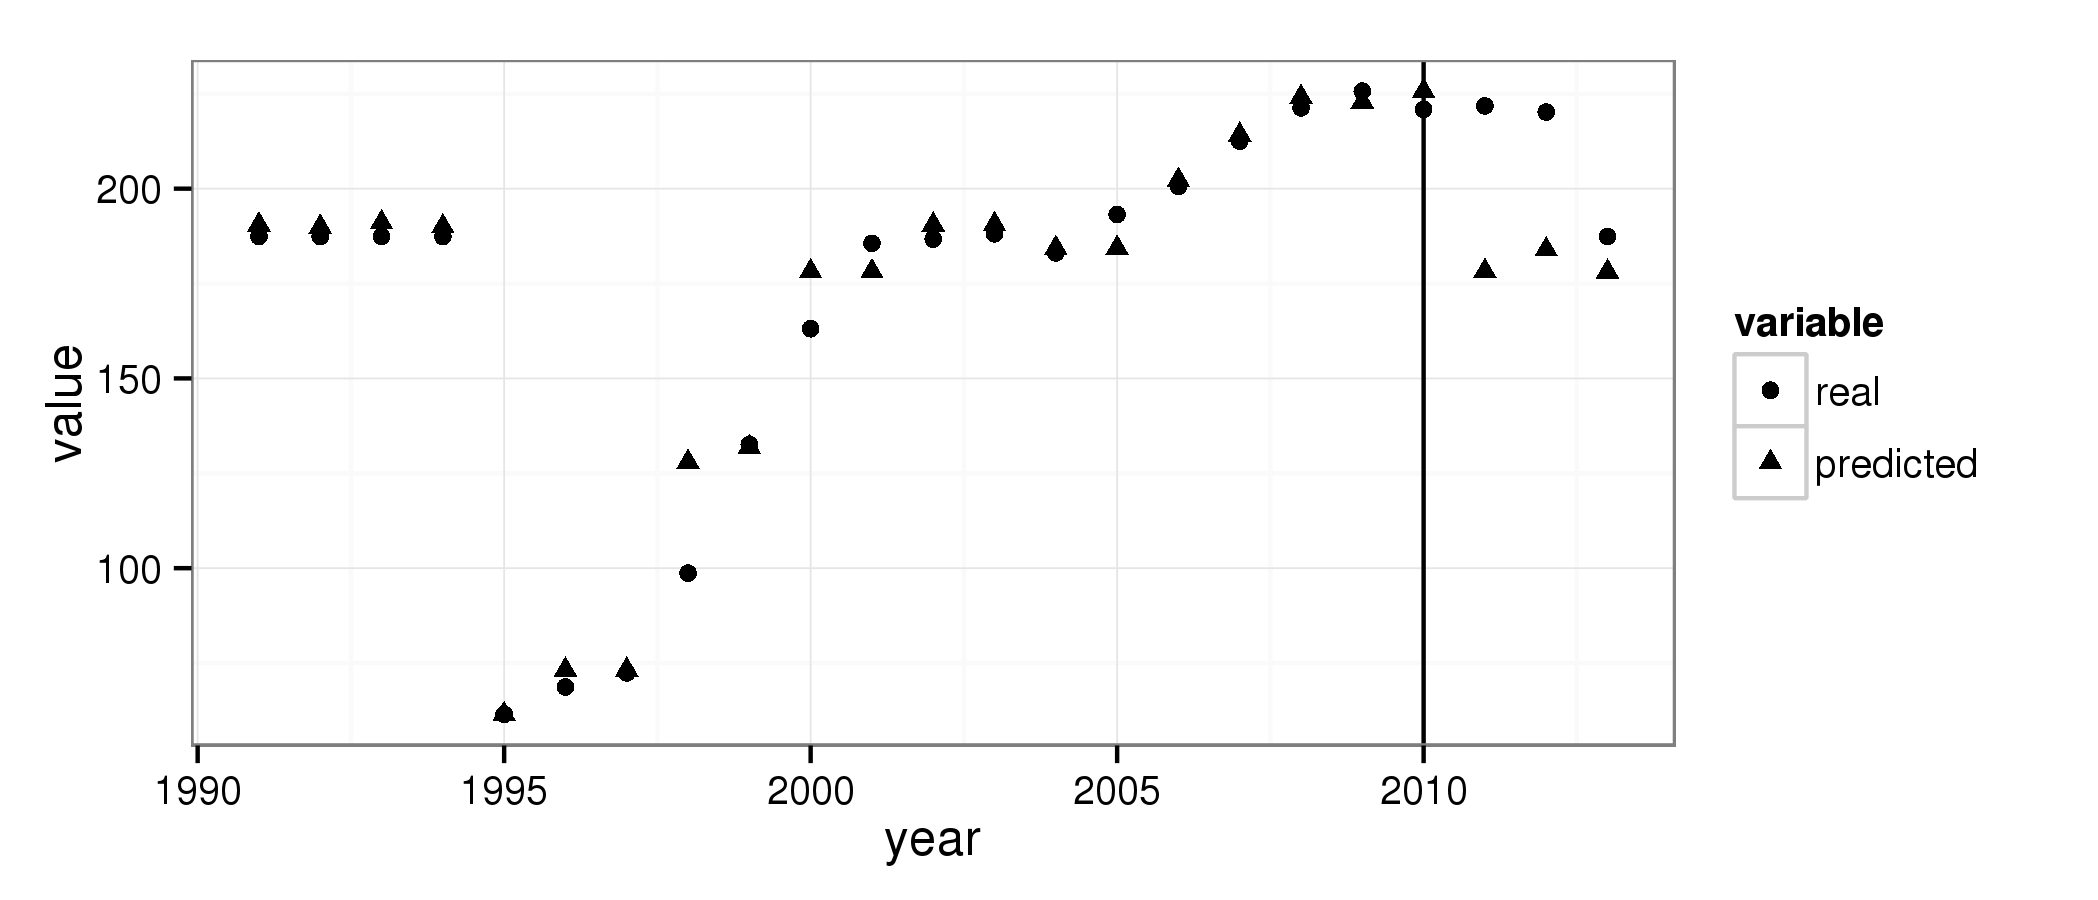
\includegraphics{images/m_plot1.png}
        \caption{Прогноз в случае (1), горизонт 3 года.}		
        \label{figure:m_plot1}
    \end{center}
\end{figure}

\begin{figure}[bhtp]
    \begin{center}
        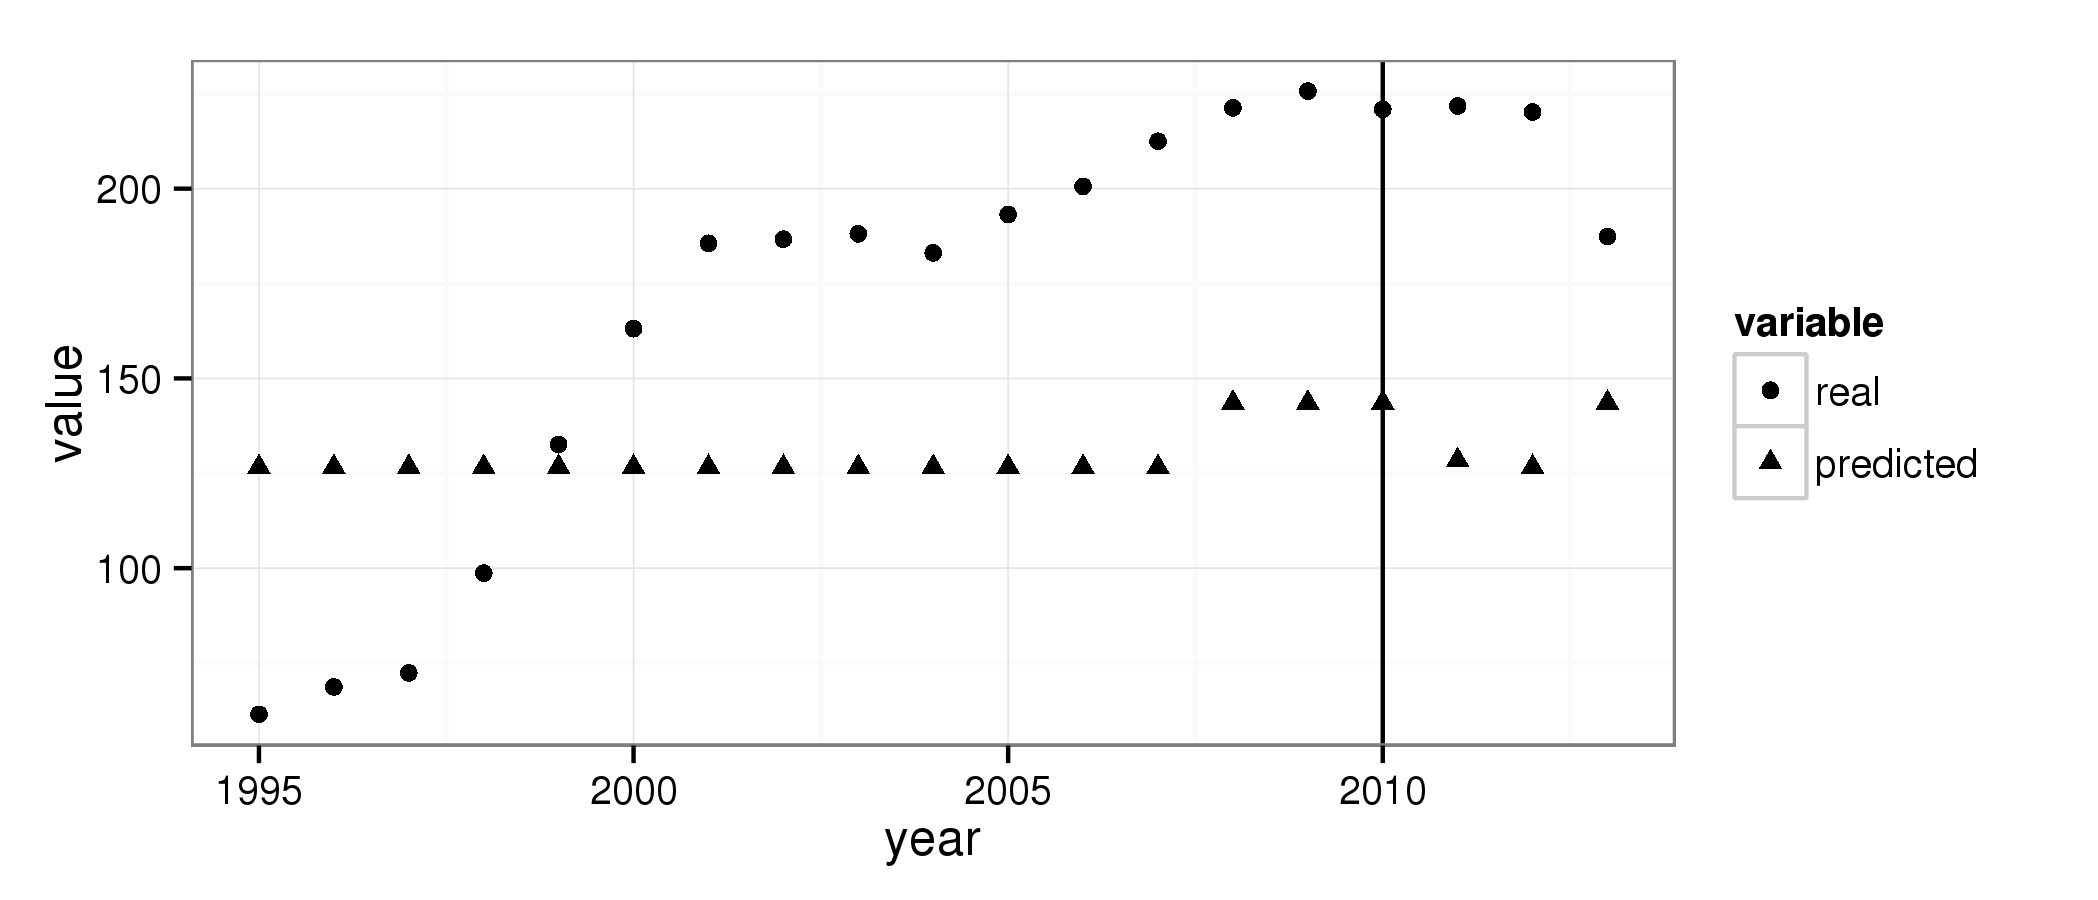
\includegraphics{images/m_plot2.png}
        \caption{Прогноз в случае (2), горизонт 3 года.}		
        \label{figure:m_plot2}
    \end{center}
\end{figure}

\begin{figure}[bhtp]
    \begin{center}
        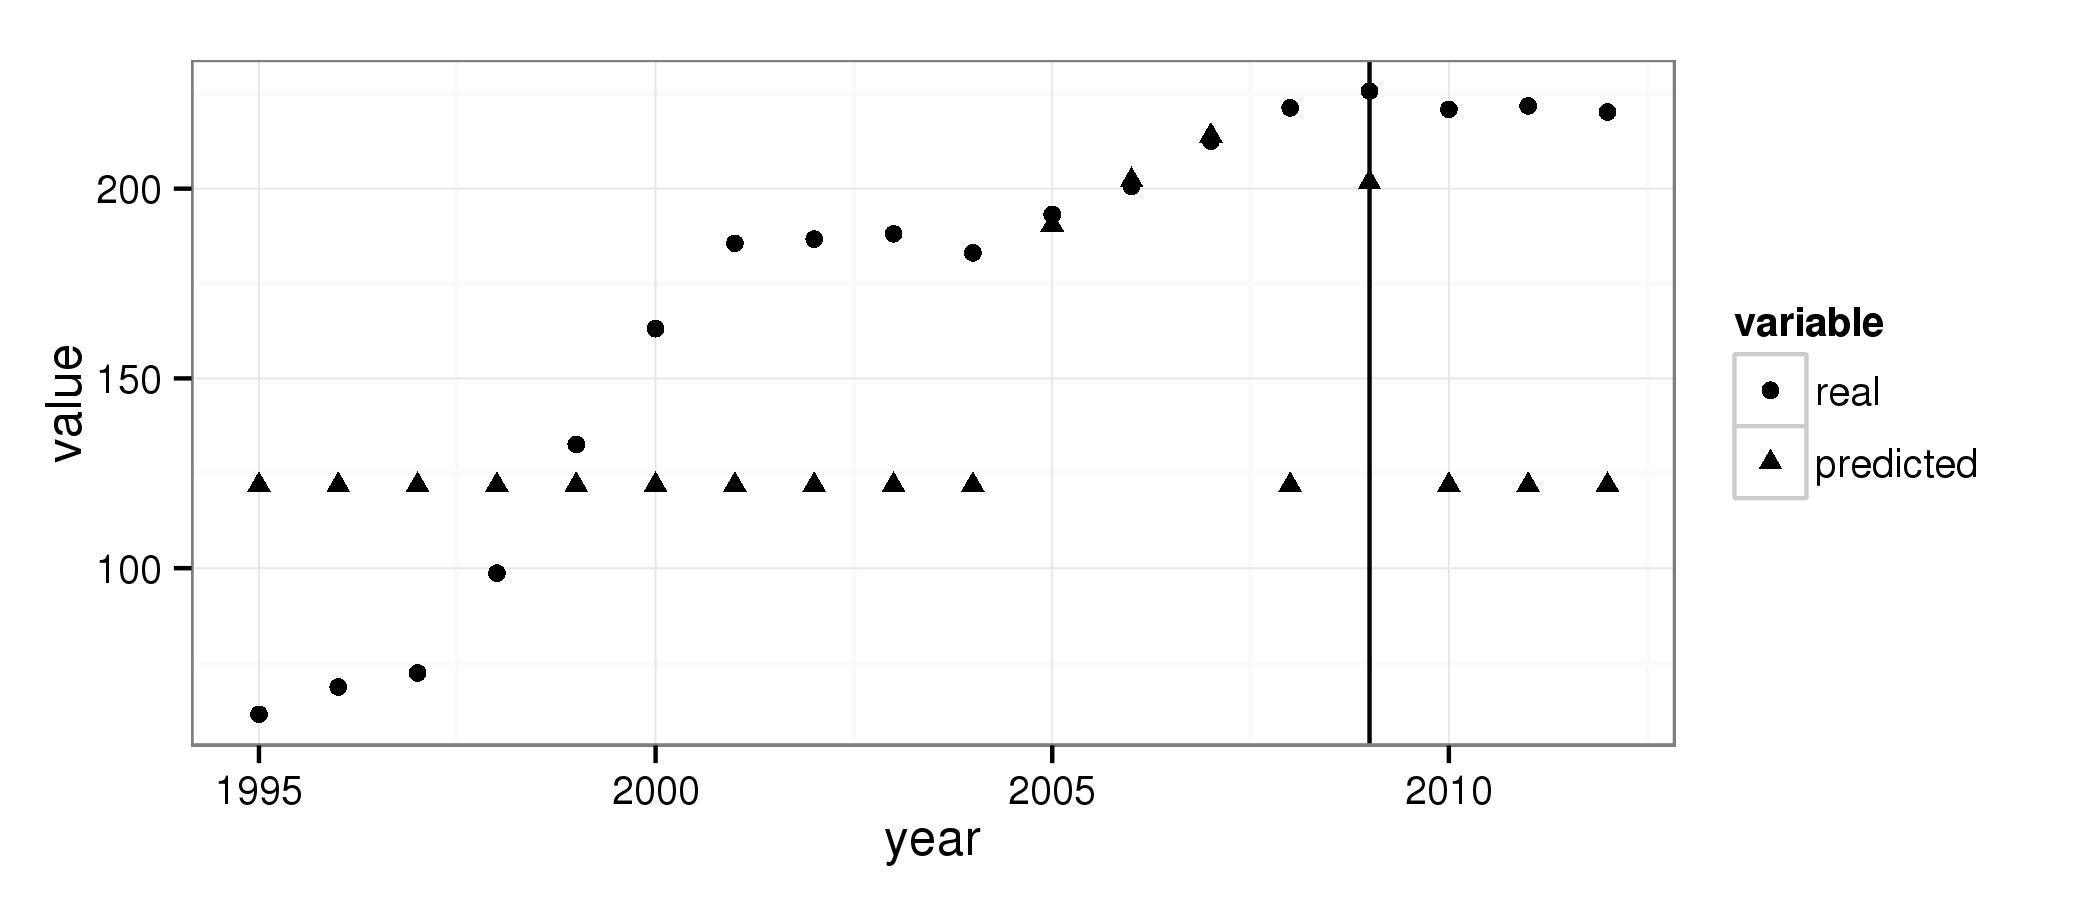
\includegraphics{images/m_plot3.png}
        \caption{Прогноз в случае (3), горизонт 3 года.}		
        \label{figure:m_plot3}
    \end{center}
\end{figure}

С точки зрения точности прогноза, в случае (1) наблюдается существенное 
улучшение относительно одномерного варианта. 
Однако, требуемый уровень точности на данный момент не 
достигнут.

Низкие оценки точности прогноза в случаях (2) и (3) объясняются, по мнению 
автора, неполнотой исходных данных, которая выражается в наличии пропущенных 
значений в независимых переменных, требующих их экстраполяции (в нашем случае 
для заполнения пропусков использовалась функция медианы), что заведомо снижает 
количество доступной для модели информации, и искажает характеристики случайных 
величин, тем самым нарушая механизмы прогнозирования.

\newpage
\section*{Заключение}
\addcontentsline{toc}{section}{Заключение}

В работе был проведен обзор видов наркополитик, в общем виде описывающих 
концептуальные основы и практические меры по урегулированию наркоситуации.  
Исследована связь между постулируемыми в странах стратегиями антинаркотической 
политики и средствами её информационной поддержки.

Экспериментальная часть данного исследования была направлена на сравнение 
точности прогнозной модели при использовании разных входных индикаторов 
наркоситуации.  Согласно результатам эксперимента, наблюдается значительное 
улучшение точности при условии достаточного объема и низкой зашумленности 
исходных данных. 

Приоритетными направлениями дальнейшей деятельности являются:
\begin{itemize}
    \item Более тщательный и полный выбор показателей для прогнозирования. 
        (Возможно использование данных в разрезе по полу, возрасту; разбивка 
        временных рядов на месяца вместо годов и т.п.);
    \item Обеспечение стабильно-высокой точности прогноза;
    \item Интеграция модели прогнозирования в <<ИС ИАО>>.
\end{itemize}

\newpage
\printbibliography[heading=bibintoc]

\end{document} % конец документа

